\chapter{Object detection and segmentation}
In this thesis we focus on tracking objects in video data using target tracking algorithms with dynamic detection probability due to the existence of obstacles that cause sensors to not detect objects in certain situations. But first, we need to have a sensor to detect objects in a
frame.


\section{Object detection}
Object detection is a fundamental task in computer vision that involves identifying and localizing objects
within images or video frames, respectively. Unlike image classification, which assigns a single label to an entire
image, object
detection algorithms aim to detect multiple objects of various classes and localize them with bounding boxes.
Alongside image classification and object detections, there are other tasks, such as semantic segmentation and
instance segmentation. Figure \ref{fig:seg_type} shows differences between these types of image processing tasks.

\begin{figure}
  \centering
  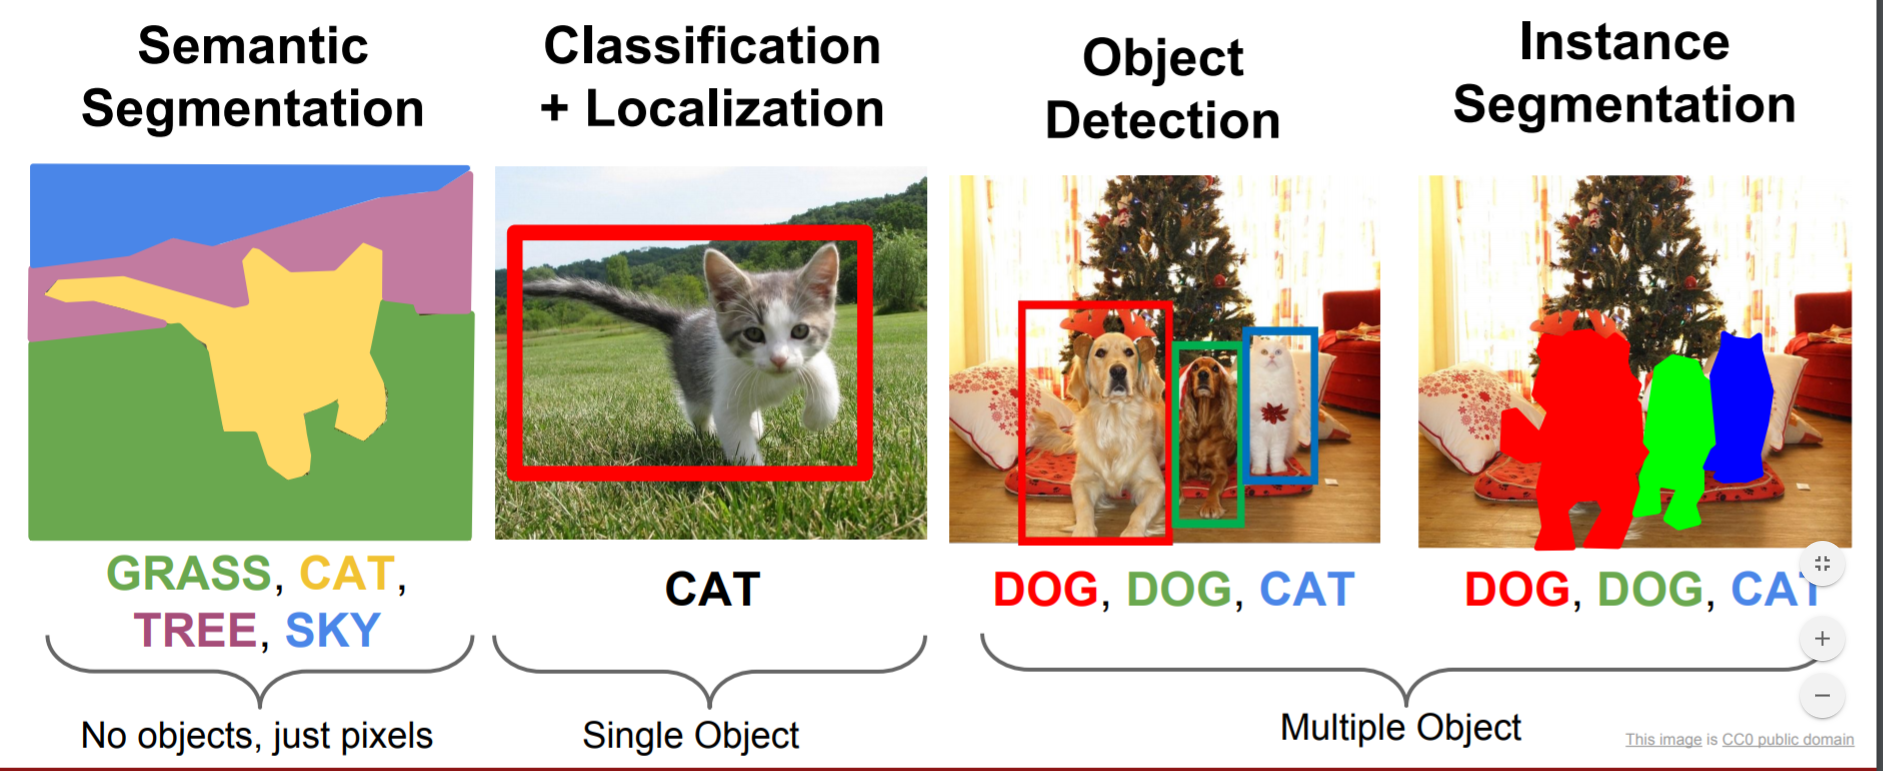
\includegraphics[width=\linewidth]{text/chapter_03/imgs/segmentation-types}
  \caption{Image detection and segmentation task types. (Source: \href{https://techvidvan.com/tutorials/image-segmentation-machine-learning/}{techvidvan.com}.)}
  \label{fig:seg_type}
\end{figure}

The development of object detection algorithms has evolved significantly over the years, driven by advances in deep
learning, dataset availability and computational power. Traditional object detection methods relied on handcrafted
features and machine learning algorithms, such as sliding window-based classifiers, histogram of oriented gradients (HOG) \cite{HoOGDalal2005}, and Haar cascades \cite{HaarCascadesLi2016}. While effective in certain scenarios, these methods often lacked robustness and scalability, particularly in complex and cluttered scenes.

With the advent of deep learning, convolutional neural networks (CNNs) improved the field of object detection. CNNs are
capable of automatically learning hierarchical representations of data, making them well suited for image analysis
tasks. The rise of CNN-based approaches has led to significant improvements in object detection accuracy and efficiency.
At its core, a convolutional neural network is comprised of multiple layers, each designed to perform specific operations on input data, typically images. The fundamental layers in a CNN include convolutional layers, pooling layers, and fully connected layers.
\begin{enumerate}
  \item \textbf{Convolutional layers:} These layers are responsible for extracting features from the input data. They consist of filters (also called kernels) that slide across the input image, performing a mathematical operation known as convolution. Each filter detects certain patterns or features, such as edges, textures, or shapes. By convolving the filters with the input image, the CNN can capture hierarchical representations of features, starting from simple edges and gradients to more complex structures.
  \item \textbf{Pooling layers:} Pooling layers are interspersed between convolutional layers to reduce the spatial dimensions of the feature maps while retaining important information. Common pooling operations include max pooling and average pooling, which downsample the feature maps by taking the maximum or average value within each pooling region. This downsampling helps in reducing computational complexity and controlling overfitting by enforcing spatial invariance.
  \item \textbf{Fully connected layers:} These layers are typically placed at the end of the CNN and serve to classify the features extracted by the convolutional layers. Each neuron in a fully connected layer is connected to every activation in the previous layer, forming a dense network. These layers use techniques like softmax activation to produce probability distributions over the classes in a classification task or regression outputs in a regression task.
\end{enumerate}
It is important to note, that it is common to combine more convolutional, pooling and fully connected layers with differently sized kernels in the architecture to improve the performance. Example of such architecture is shown in Figure \ref{fig:CNNArchitecture}
\begin{figure}
  \centering
  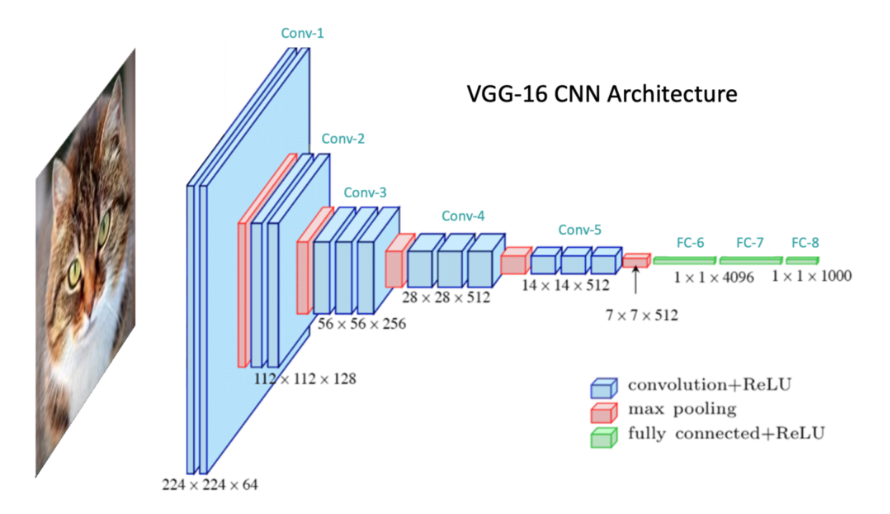
\includegraphics[width=\linewidth]{text/chapter_03/imgs/CNN}
  \caption{CNN architecture example. (Source \href{https://learnopencv.com/understanding-convolutional-neural-networks-cnn/}{learnopencv.com})}
  \label{fig:CNNArchitecture}
\end{figure}
During training, CNNs use a process called backpropagation to adjust the parameters (weights and biases) of the network based on the disparity between the predicted outputs and the ground truth labels. This optimization process aims to minimize a predefined loss function, such as cross-entropy loss for classification tasks or mean squared error for regression tasks. By iteratively updating the parameters using optimization algorithms like stochastic gradient descent (SGD) or its variants, CNNs gradually learn to recognize and classify patterns within the input data, ultimately improving their performance on various visual tasks such as object detection and segmentation.


Object detection poses several challenges, including variations in object appearance, scale, orientation, occlusion, and cluttered backgrounds. Additionally, real-world images often contain multiple objects of different classes, making it essential for detection algorithms to handle overlapping and partially visible objects.

Furthermore, object detection systems often have to balance accuracy and speed to meet the demands of real-time
applications. Achieving high detection accuracy while maintaining fast inference times is a fundamental challenge,
especially for devices with low hardware resources and applications requiring low-latency processing.

Object detection algorithms typically consist of several components:

\begin{itemize}
  \item \textbf{Input processing:} Images or video frames are preprocessed to standardize their format and size, often
involving resizing, normalization, and data augmentation to enhance model generalization.
  \item \textbf{Feature extraction:} Feature extraction is performed to capture relevant information from the input
  data. In deep learning-based approaches, convolutional neural networks are commonly used to extract hierarchical features that encode object appearance and spatial relationships.
  \item \textbf{Localization:} Localization involves predicting the spatial extent of objects within the image using
bounding boxes. This step requires regression or classification to estimate bounding box coordinates and confidence scores for object presence.
  \item \textbf{Classification:} Object classification assigns class labels to detected objects based on their visual
  appearance. Classification models are trained to distinguish between different object categories, enabling accurate identification of objects within the scene.
  \item \textbf{Post-processing:} Post-processing techniques, such as non-maximum suppression (NMS), are applied to
  refine detection results, suppress duplicate detections, and improve localization accuracy.
\end{itemize}



  \subsection{YOLO}

In the realm of object detection, the emergence of You Only Look Once (YOLO) represents a paradigm shift, propelled by the fusion of deep learning and innovative architectural design. YOLO stands as a testament to the transformative power of convolutional neural networks (CNNs) in redefining the landscape of computer vision applications, particularly in real-time object detection scenarios. This object detector was proposed by Developed by Joseph Redmon, Santosh Divvala, Ross Girshick, and Ali Farhadi in \cite{YOLORedmon2016}.

At its core, YOLO introduces a groundbreaking concept: the ability to predict bounding boxes and class probabilities for objects within an image in a single pass through the neural network. This departure from traditional object detection methods, which often involve multi-stage processes and post-processing steps, marks a significant leap forward in efficiency and speed. By consolidating object localization and classification into a unified framework, YOLO streamlines the detection pipeline, enabling seamless integration into various applications requiring rapid decision-making based on visual data.


A distinguishing feature of YOLO lies in its holistic approach to image analysis. Unlike conventional methods that segment images into regions of interest for further processing, YOLO takes a global perspective by dividing the input image into a grid and processing it as a whole. This global context consideration not only enhances the model's understanding of spatial relationships but also reduces the risk of misclassification, particularly in complex scenes with multiple objects. Each bounding box prediction includes coordinates $(x, y)$ for the center of the box, width, height, and confidence score indicating the likelihood of containing an object. Additionally, class probabilities are estimated for each bounding box to determine the object category. YOLO employs a loss function that penalizes localization errors, confidence errors, and classification errors.
This loss function is optimized during training using labeled datasets to learn accurate object representations. Moreover, YOLO adopts anchor boxes to improve localization accuracy and handle scale variations of objects within the image.

The evolution of YOLO over successive versions underscores its adaptability to diverse use cases and computational environments. While early iterations prioritized speed, subsequent iterations like YOLOv4 and YOLOv5 have aimed to enhance accuracy without compromising real-time performance \cite{YoloVersions2022}. This flexibility in model selection empowers users to tailor YOLO to their specific requirements, whether it be for surveillance systems demanding rapid detection or autonomous vehicles requiring precise object localization.

Compared to traditional object detection methodologies such as region-based convolutional neural networks (R-CNN) \cite{MaskRCNN2017} and single-shot detectors (SSD), YOLO stands out for its simplicity and efficiency. By eliminating the need for complex post-processing steps and leveraging a unified architecture for object detection (see Figure \ref{fig:yoloArchitecture} for YOLO architecture), YOLO achieves a fine balance between speed and accuracy. This versatility extends YOLO's applicability across a myriad of domains, including but not limited to autonomous driving, industrial automation, healthcare imaging, and augmented reality.

\begin{figure}
  \centering
  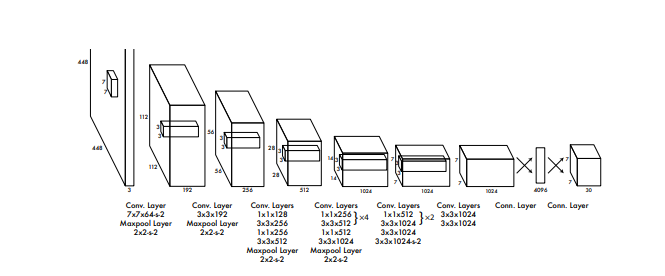
\includegraphics[width=\linewidth]{text/chapter_03/imgs/YOLO_architecture}
  \caption{Yolo architecture proposed in \cite{YOLORedmon2016} has 24 convolutinal layers followed by 2 fully connected layers. Convolutional layers were pretrained on the ImageNet classificator at half resolution (224 x 224 input image) and the doubled the resolution for detection. (Source \cite{YOLORedmon2016}.)}
  \label{fig:yoloArchitecture}
\end{figure}


\section{Image segmentation}
Image segmentation, a fundamental technique in computer vision, involves dividing a digital image into distinct pixel groups called segments. By breaking down the visual data into manageable segments, image segmentation facilitates more efficient and sophisticated image processing.

The methods employed for image segmentation vary from straightforward heuristic approaches to cutting-edge deep learning techniques. Traditional algorithms typically analyze basic visual attributes such as color and brightness to delineate object boundaries and background regions. Machine learning plays a pivotal role in this domain by training models on labeled datasets, allowing them to accurately classify objects and regions within images.

With its versatility and practical applications, image segmentation finds widespread use across artificial intelligence scenarios. Its applications span from assisting medical diagnoses through imaging to enabling automation in robotics and self-driving vehicles. Furthermore, it plays a crucial role in tasks such as identifying objects within satellite imagery.

There are three main task types in image segmentation: semantic segmentation, instance segmentation and panoptic segmentation \cite{IBM}.
The distinction between various types of image segmentation tasks hinges on how they handle semantic classes, which are specific categories assigned to individual pixels within an image.

In the realm of computer vision, semantic classes are broadly categorized into two types, each requiring distinct segmentation techniques for accurate results.
\begin{itemize}
  \item \textit{Things} represent classes of objects characterized by identifiable shapes, such as \textit{car, tree,} or \textit{person}. These classes typically consist of discrete instances with consistent sizes and distinguishable constituent parts. For instance, all cars have wheels, which are distinct from the car itself.
  \item \textit{Stuff} refers to semantic classes with amorphous shapes and variable sizes, like sky, water, or grass
  . Unlike \textit{things}, \textit{stuff} lacks clearly defined, countable individual instances and does not possess distinct parts. For example, both a single blade of grass and an entire field of grass fall under the category of \textit{grass}.
\end{itemize}
In certain image contexts, some classes can straddle the line between being considered \textit{things} or \textit{stuff}. For instance, a large gathering of people might be interpreted either as multiple people -- each being a clearly shaped, countable thing, or as a singular, indistinct person.

While much of the focus in object detection typically centers on \textit{thing} classes, it is crucial to recognize that \textit{stuff}, such as sky, walls, floors, and ground constitutes the bulk of our visual environment. \textit{Stuff} serves as crucial contextual information for identifying \textit{things}. For instance, a metallic object on the road is likely a car, while a blue background behind an object is indicative of water if it is a boat or sky if it is a plane. This interplay between \textit{stuff} and \textit{things} holds particular significance for deep learning models.

  \subsection{Semantic segmentation}
Semantic segmentation represents the most straightforward form of image segmentation. In this approach, a semantic segmentation model assigns a semantic class to every pixel in an image, without providing additional context or information, such as the identification of specific objects.

Unlike more nuanced segmentation techniques, semantic segmentation treats all pixels uniformly as \textit{stuff} without distinguishing between \textit{stuff} and \textit{things}. This means that it does not differentiate between different types of objects within the same class.

For instance, imagine a semantic segmentation model trained to analyze urban scenes. It would generate segmentation masks outlining the boundaries of various classes of \textit{things} and \textit{stuff}. However, it would not differentiate between individual instances of the same class. For example, if there are multiple trees in a forest, the model would likely treat them as one continuous tree segment rather than recognizing each individual tree separately.

\subsection{Instance segmentation}
Instance segmentation represents a departure from the approach of semantic segmentation. While semantic segmentation focuses solely on assigning semantic classes to each pixel without distinguishing between individual instances, instance segmentation precisely outlines the shape of each separate object instance within an image.

In essence, instance segmentation segregates \textit{things} from \textit{stuff}, disregarding the latter, and can be viewed as a more sophisticated version of object detection. Instead of providing rough bounding boxes, instance segmentation furnishes precise segmentation masks for each object instance.

This task poses greater challenges compared to semantic segmentation. Even when instances of the same class overlap or touch each other, instance segmentation models must accurately separate and delineate the shape of each instance. In contrast, semantic segmentation models may simply group them together.

Instance segmentation algorithms typically adopt either a two-stage or one-shot methodology to address the task.

Two-stage models, exemplified by Region-based Convolutional Neural Networks \cite{RCNN2014}, initially conduct conventional object detection to produce bounding boxes for each potential instance. Subsequently, they refine segmentation and classification within these bounding boxes to precisely delineate each object instance.

Conversely, one-shot models, such as YOLO, streamline the process by simultaneously performing object detection, classification, and segmentation. This approach enables real-time instance segmentation.

While one-shot methods boast faster processing speeds, they often sacrifice some accuracy. On the other hand, two-stage approaches prioritize accuracy but may be slower due to the additional refinement steps.

  \subsection{Panoptic segmentation}
Panoptic segmentation represents a synthesis of semantic and instance segmentation methodologies, offering a comprehensive understanding of an image.

In panoptic segmentation, each pixel receives both a semantic label and an instance ID. Pixels with the same label and ID are assigned to the same object instance. For \textit{stuff} pixels, the instance ID is disregarded.

This approach provides computer vision systems with a complete and cohesive interpretation of an image, combining the benefits of both semantic and instance segmentation. However, achieving panoptic segmentation consistently and efficiently presents significant computational challenges. Despite its evident appeal, realizing panoptic segmentation in a manner that balances accuracy and computational efficiency remains a formidable task.

The challenge in achieving panoptic segmentation lies in reconciling the conflicting approaches of semantic and instance segmentation models. Semantic segmentation treats all pixels uniformly as \textit{stuff}, disregarding individual instances of objects, while instance segmentation focuses solely on isolating individual objects, ignoring \textit{stuff}. Integrating these methodologies proves difficult as neither model can effectively take on the responsibilities of the other.

Early attempts at panoptic segmentation involved combining separate semantic and instance segmentation models, followed by a post-processing phase to merge their outputs. However, this approach encountered two significant drawbacks: it demanded substantial computational resources and struggled with inconsistencies between the data produced by the semantic segmentation network and that produced by the instance segmentation network.

Recent advancements in panoptic segmentation architectures aim to overcome these limitations through a more unified deep learning approach. Many of these architectures utilize a common backbone network, such as a feature pyramid network (FPN) \cite{FPNLin2017}, to extract features from the input image. These features are then fed into parallel branches, such as a foreground branch and a background branch, or a semantic head and an instance head. The outputs from each branch are merged using a weighted system to produce the final segmentation. Notable proposed architectures include EfficientPS \cite{mohan2020efficientps}, OANet \cite{zhang2019oanet}, PanopticFPN \cite{kirillov2019panoptic}, UPSNet \cite{xiong2019upsnet}, SOGNet \cite{yang2019sognet}, BGRNet \cite{wu2020bidirectional}, AUNet \cite{sun2019aunet} and others.

\subsection{Traditional image segmentation}
Traditional image segmentation techniques leverage pixel color values and related characteristics, such as brightness, contrast, or intensity, for feature extraction. These methods are often trained with simple machine learning algorithms and are particularly useful for tasks like semantic classification. Despite their limitations in precision compared to deep learning-based approaches, traditional methods offer advantages in terms of lower cost and computational demands, allowing them to efficiently solve certain problems.

Some common traditional image segmentation techniques include:
\begin{enumerate}
  \item \textbf{Thresholding:} Thresholding methods create binary images by classifying pixels based on whether their intensity exceeds or falls below a predetermined threshold value. Otsu's method is frequently used to identify the threshold value that minimizes intra-class variation \cite{otsu1979}.
  \item \textbf{Histograms:} Histograms plot the frequency of specific pixel values in an image and are often employed to define thresholds. For instance, histograms can infer background pixel values, aiding in the isolation of object pixels.
  \item \textbf{Edge detection:} Edge detection techniques identify object boundaries or classes by detecting abrupt changes in brightness or contrast \cite{Edgedet1986}.
  \item \textbf{Watersheds:} Watershed algorithms \cite{Watershed1991} convert images to grayscale and generate a topographic map where each pixel's elevation is determined by its brightness. Regions, boundaries, and objects can be inferred from the formation of valleys, ridges, and catchment basins.
  \item \textbf{Region-based segmentation:} Region-growing algorithms \cite{RCNN2016} initiate segmentation with one or more seed pixels, progressively grouping neighboring pixels with similar characteristics. These algorithms can be either agglomerative or divisive.
  \item \textbf{Clustering-based segmentation:} Clustering algorithms \cite{ClusteringSeg1979}, an unsupervised learning technique, partition visual data into clusters of pixels with similar values. One popular variant is K-means clustering, where k represents the number of clusters. In this method, pixel values are treated as data points, and $k$ random points are selected as the centroids of clusters. Each pixel is then assigned to the nearest centroid based on similarity. Centroids are iteratively relocated to the mean of each cluster until convergence, resulting in stabilized clusters.
\end{enumerate}

\subsection{Deep learning image segmentation}
Trained on meticulously annotated datasets, deep learning image segmentation models harness the power of neural networks to uncover underlying patterns within visual data. These models discern salient features crucial for tasks such as classification, detection, and segmentation.

Despite their higher computational requirements and longer training times, deep learning models consistently outperform traditional approaches, serving as the cornerstone for ongoing advancements in computer vision.

Some prominent deep learning models utilized in image segmentation include:

\begin{enumerate}
  \item \textbf{Fully Convolutional Networks:} FCNs \cite{FCNLong2015}, commonly employed for semantic segmentation, are a
  variant
  of
  convolutional neural networks characterized by flexible layers. In FCNs, an encoder network processes visual input through convolutional layers to extract pertinent features for segmentation or classification. The compressed feature data is then passed through decoder layers to upsample and reconstruct the input image along with segmentation masks.
  \item \textbf{U-Nets:} U-Nets \cite{ronneberger2015unet} adapt the FCN architecture to mitigate data loss during downsampling by
  incorporating skip connections. These connections enable the preservation of finer details by selectively bypassing
  certain convolutional layers as information propagates through the network. The name U-Net derives from the shape 
  of diagrams illustrating its layered arrangement (see Figure \ref{fig:unet_architecture}).
  \item \textbf{Deeplab:} Similar to U-Nets, Deeplab modifies the FCN architecture \cite{Deeplab2018}. In addition to utilizing skip
  connections, Deeplab employs dilated (or "atrous") convolution to produce larger output maps without requiring additional computational resources.
  \item \textbf{Mask R-CNNs:} Mask R-CNNs stand out as a leading model for instance segmentation \cite{MaskRCNN2017}. These models
  integrate a region proposal network (RPN), responsible for generating bounding boxes for potential instances, with an FCN-based "mask head" that produces segmentation masks within each confirmed bounding box.
  \item \textbf{Transformers:} Inspired by the success of transformer models \cite{vaswani2023attention} in natural language processing,
  newer models like the Vision Transformer (ViT) employ attention mechanisms in lieu of convolutional layers. These models have demonstrated comparable or superior performance to CNNs for various computer vision tasks.
\end{enumerate}

\begin{figure}
  \centering
  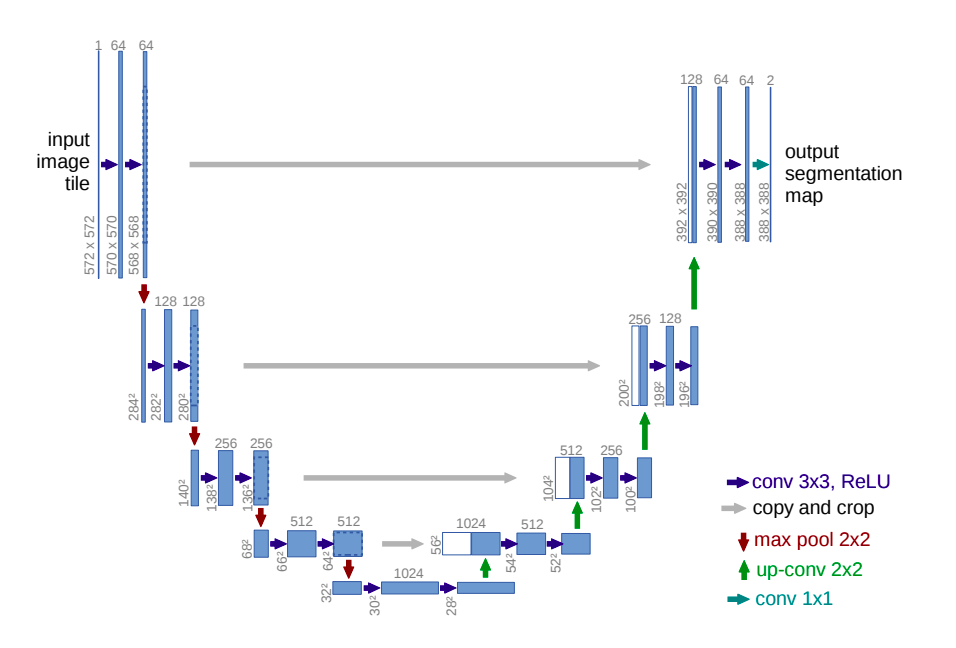
\includegraphics[width=\linewidth]{text/chapter_03/imgs/unet}
  \caption{U-net architecture (example for 32x32 pixels in the lowest resolution). (Source \cite{ronneberger2015unet})}
  \label{fig:unet_architecture}
\end{figure}

\subsubsection{Transformers}
As we use Transformer model in our work, we briefly demonstrate Transformers' architecture and how they work.
Transformers consist of a stack of identical layers, typically comprising an encoder and a decoder (Figure \ref{fig:transformer_architecture}). The
encoder
processes the input sequence, while the decoder generates the output sequence.


\begin{figure}
  \centering
  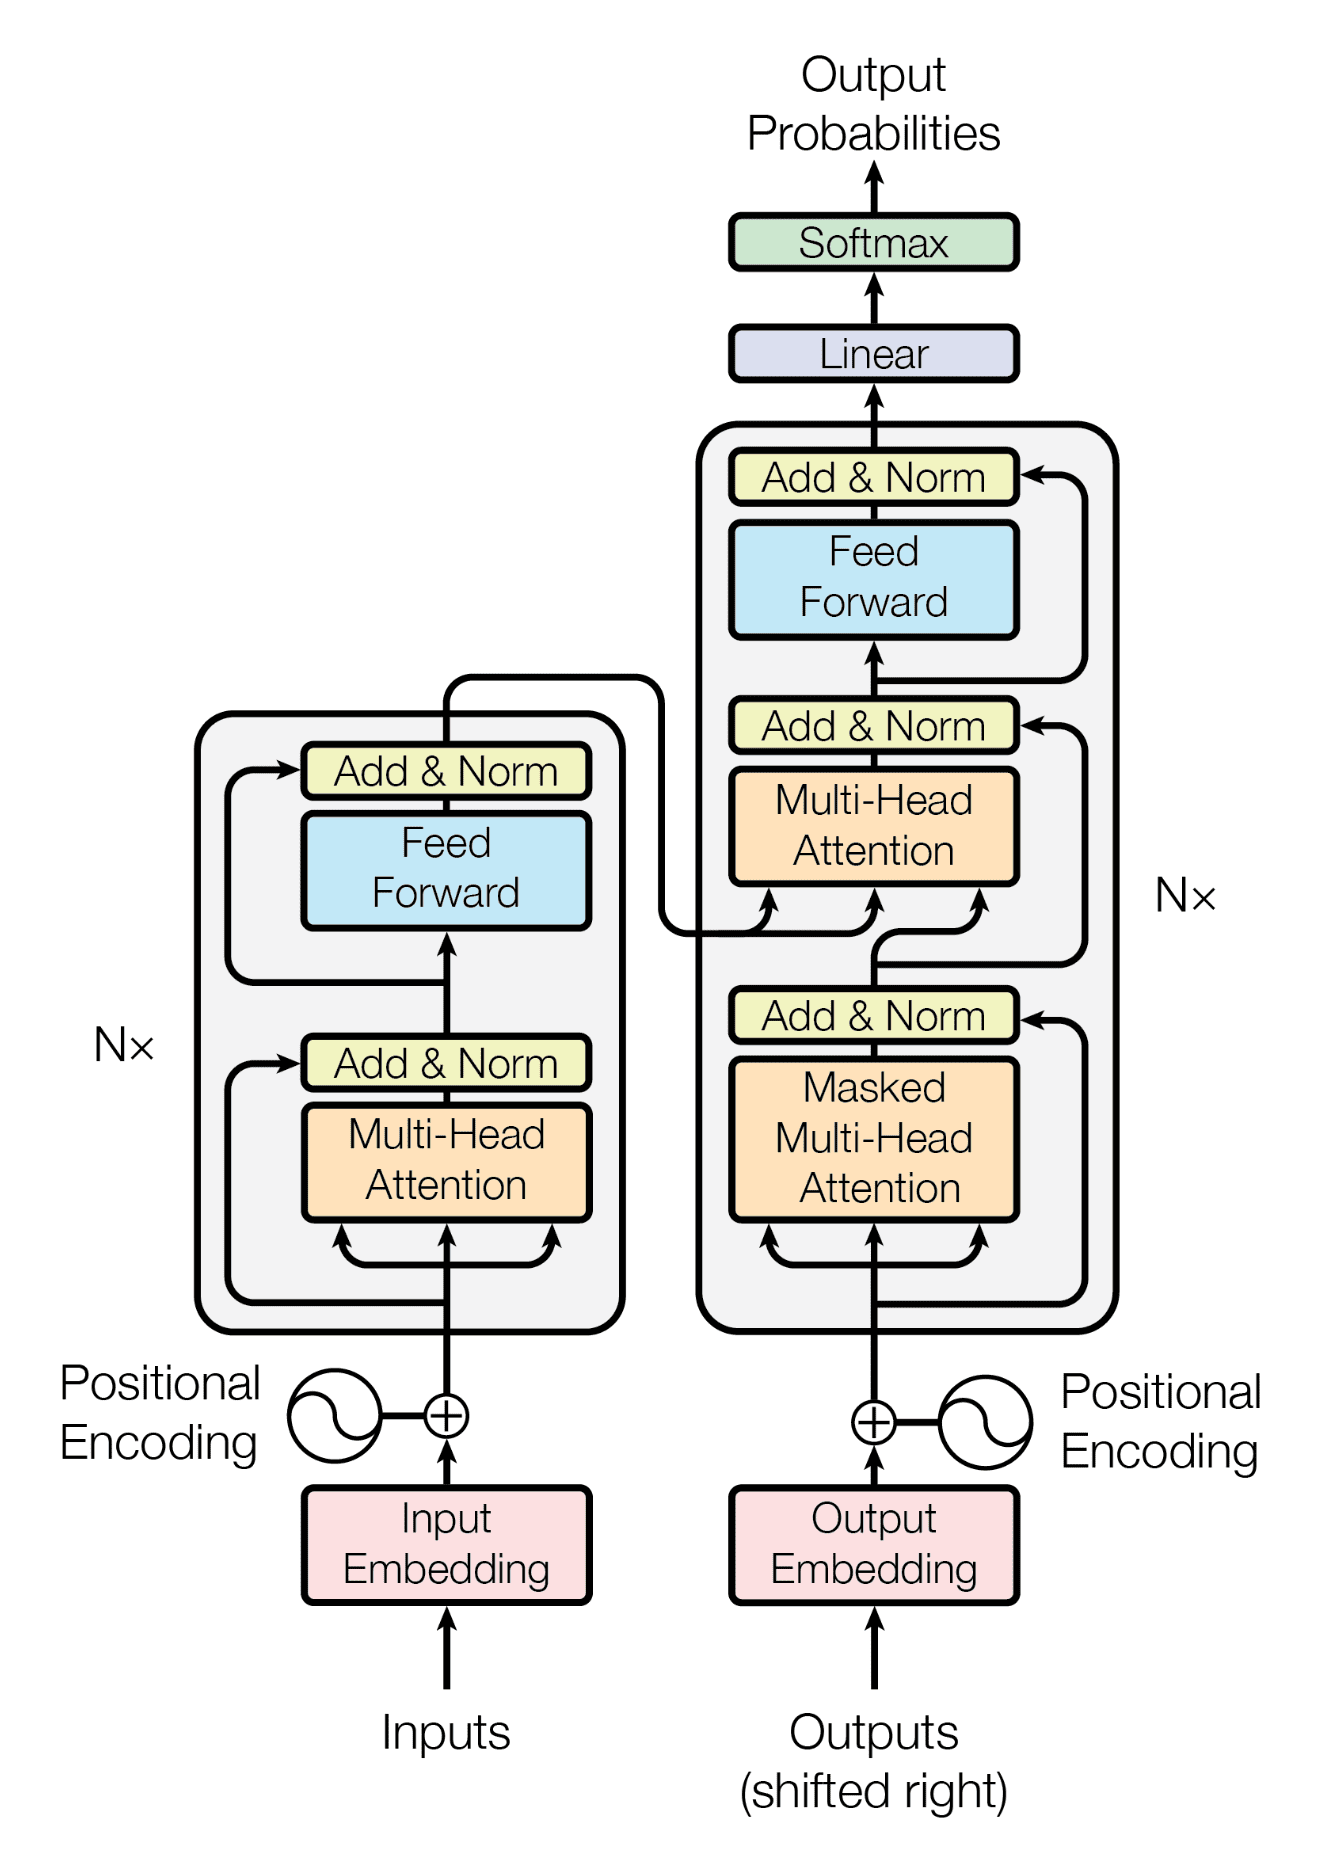
\includegraphics[width=0.5\linewidth]{text/chapter_03/imgs/transformers}
  \caption{Transformer architecture. (Source \cite{vaswani2023attention})}
  \label{fig:transformer_architecture}
\end{figure}

\begin{itemize}
  \item \textbf{Encoder:} The encoder is composed of a stack of $N=6$ identical layers. Each layer has two
  sub-layers. The first is a multi-head self-attention mechanism (Figure \ref{fig:transformer_multihead}), and the second is positionwise fully
  connected feed-forward network. There is a residual connection \cite{DeepResidual2016} around each of two sub-layers, followed by normalization \cite{ba2016layer}: the output of each sub-layer is $LayerNorm(x + Sublayer(x))$, where $Sublayer(x)$ is the function implemented by the sub-layer
  itself.
  \item \textbf{Decoder:} The decoder is also composed of a stack of $N=6$ identical layers. In addition to the two
  sub-layers in each encoder layer, the decoder inserts a third sub-layer, which performs multi-head
  attention over the output of the encoder stack. Similar to the encoder, there is residual connections
  around each of the sub-layers, followed by layer normalization.
\end{itemize}

\begin{figure}
  \centering
  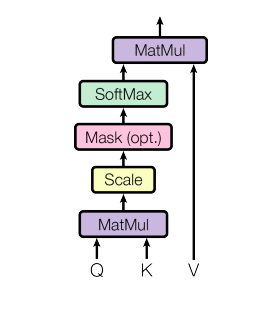
\includegraphics[width=0.5\linewidth]{text/chapter_03/imgs/multihead}
  \caption{Multi-head attention. (Source \cite{vaswani2023attention})}
  \label{fig:transformer_multihead}
\end{figure}


The core of the Transformer architecture lies in its self-attention mechanism \cite{vaswani2023attention}. This mechanism enables each token in the input sequence to attend to every other token, learning contextual relationships and dependencies. By computing attention scores between all pairs of tokens and taking weighted sums of their embeddings, the Transformer can effectively capture long-range dependencies and dependencies between distant tokens.

To enhance the expressiveness of self-attention, Transformers employ multi-head attention mechanisms. Instead of computing attention once, multi-head attention computes attention multiple times in parallel, each with its set of learnable parameters. This allows the model to attend to different aspects of the input sequence simultaneously, facilitating richer representations and improved performance.

Unlike sequential models, Transformers do not inherently encode the positional information of tokens. To address this limitation, positional encoding is added to the input embeddings to convey the position of each token in the sequence. This positional information is crucial for the Transformer to distinguish between tokens with the same content but different positions within the sequence.

In addition to self-attention layers, Transformers incorporate feedforward neural networks within each layer. These FNNs consist of multiple fully connected layers with non-linear activation functions, enabling the model to capture complex interactions and transformations within the input data
\begin{align}
  FFN(x) &= max(0, xW_1 + b_1)W_2 + b_2,
\end{align}
where $W$ are weights and $b$ stands for bias.

To stabilize training and facilitate gradient flow, Transformers employ layer normalization and residual connections within each layer. Layer normalization normalizes the activations across feature dimensions, while residual connections enable the direct flow of gradients through the network, mitigating the vanishing gradient problem.

During training, Transformers are optimized using backpropagation and gradient-based optimization algorithms, such as
Adam \cite{kingma2017adam} or SGD \cite{rakhlin2012making}, to minimize a predefined loss function. By iteratively updating the
parameters of the model based on
the disparity between the predicted outputs and the ground truth labels, Transformers learn to encode and generate
meaningful representations of input sequences, enabling them to excel in various NLP tasks and more recently
image processing tasks.



%Object segmentation involves partitioning an image into semantically meaningful regions and associating each region with a specific object instance. Unlike object detection, which identifies objects at the bounding box level, segmentation provides pixel-level delineation of object boundaries. This fine-grained information is invaluable for tasks such as image understanding, scene understanding and image manipulation.

%Semantic segmentation assigns a class label to each pixel in the image, effectively partitioning the image into regions corresponding to different object categories. Fully Convolutional Networks (FCNs) and their variants, such as U-Net and DeepLab, have demonstrated remarkable success in semantic segmentation tasks by leveraging the power of convolutional neural networks for dense pixel-wise predictions \cite{SemanticSegmentationGuo2022}.

%Instance segmentation, on the other hand, extends semantic segmentation by distinguishing between individual object instances of the same class. This task requires not only segmenting objects but also differentiating between instances of the same class, even if they overlap or occlude each other. Mask R-CNN, an extension of Faster R-CNN, combines region-based object detection with instance segmentation, achieving state-of-the-art results in both tasks.

%Despite significant advancements, object detection and segmentation still face several challenges. These include handling scale variations, occlusions, cluttered backgrounds, and fine-grained object attributes. Additionally, achieving real-time performance while maintaining high accuracy remains a critical goal for many applications.

  \subsection{Segment anything}
To get the best possible results in practical part of this thesis, it is necessary to use powerful, yet fast image
segmentation model. The Segment Anything (SAM) model represents a significant advancement in image segmentation,
introducing a novel approach to tackling the challenges in this field \cite{SAM2023}. SAM is designed to address the need for
efficient and effective segmentation models that can generalize to diverse tasks and data distributions, even in zero-shot scenarios.

The SAM project introduces a new task, model, and dataset for image segmentation. It leverages a promptable model
architecture to achieve impressive zero-shot performance on diverse segmentation tasks. This task involves generating valid segmentation masks given any segmentation prompt. A prompt can include spatial or textual information indicating what to segment in an image. SAM ensures the output mask is reasonable for at least one interpretation of the prompt, handling ambiguity effectively.

SAM's architecture comprises three main components: an image encoder, a prompt encoder, and a mask decoder (Figure \ref{fig:sam_architecture}). The
image encoder processes input images using a Vision Transformer, while the prompt encoder handles various types of prompts, including points, boxes, and text. The mask decoder efficiently generates segmentation masks based on the input image and prompt embeddings. SAM is designed for real-time performance, enabling interactive use with low latency.

\begin{figure}[h]
  \centering
  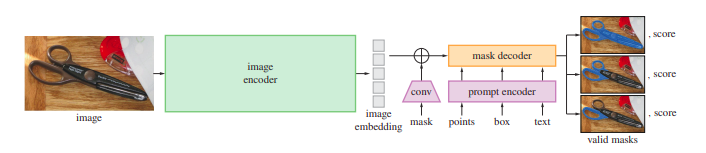
\includegraphics[width=\linewidth]{text/chapter_03/imgs/sam}
  \caption{SAM architecture (Source \cite{SAM2023})}
  \label{fig:sam_architecture}
\end{figure}

SAM addresses ambiguity by predicting multiple output masks for a single prompt. It efficiently ranks these masks based on confidence scores, allowing it to produce accurate segmentations even in complex scenarios.

Efficiency is a core consideration in SAM's design. The model's components are optimized for fast execution, enabling it to run in a web browser on CPU with a runtime of approximately 50ms. This real-time performance facilitates seamless interaction with the model for prompt-based segmentation tasks.

SAM is trained using the linear combination of focal loss \cite{FocalLoss2020} and dice loss \cite{DiceLoss2016}, tailored for the
promptable segmentation
task. It simulates an interactive setup during training, sampling prompts to ensure robustness and adaptability.

SAM's contributions include the development of a promptable segmentation task, a novel model architecture optimized
for real-time performance, and a large-scale dataset (SA-1B) comprising over 1 billion masks and 11 million images.
The model's zero-shot capabilities and efficient design make it a valuable tool for various segmentation tasks, with
potential applications across diverse domains. The example of segmented images are shown in Figure \ref{fig:sam_example}.

\begin{figure}[h]
  \centering
  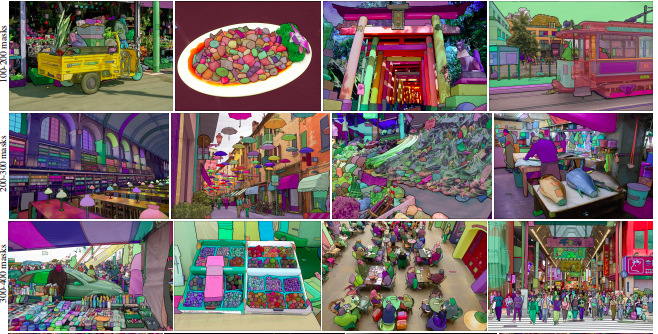
\includegraphics[width=\linewidth]{text/chapter_03/imgs/sam_example}
  \caption{The demonstration of SAM's strength. These masks were annotated fully automatically by SAM and are part of
  the SA-1B dataset. (Source \cite{SAM2023})}
  \label{fig:sam_example}
\end{figure}

\subsection{Grounded segment anything}
As SAM text prompt was not released yet,\ldots
\todo{try it}
